\section{Antecedentes}

Para entender las intenciones de la presente propuesta, es menester considerar lo que significan y representan los trámites, el gobierno electrónico y el desarrollo de software libre reutilizable. De esta manera entenderemos mejor la problemática y la solución planteada.

\subsection{El trámite}

Poco se ha escrito estrictamente sobre los trámites a nivel académico. Sin embargo, por conocimiento popular casi todos sabemos lo que son. Sabemos también lo estrechamente relacionados que están con el gobierno, la burocracia y el manejo de documentos.

La palabra trámite viene del latin \say{trames}, \say{tramitis}, que para los romanos significaba \say{senda}, \say{camino}, de donde se derivó el sentido actual de \say{vía legal o procedimiento que debe seguir una gestión}. En inglés no existe una palabra que tenga la traducción exacta de trámite, pero se usan distintas palabras como \say{Procedure}, \say{Transaction} o \say{Paperwork}. También en español se puede referir al mismo como \say{Procedimiento administrativo}. En todas estas definiciones se tienen como común denominador: Proceso, Camino, Papeleo.

Los estados requieren de su población cumplir con una serie de obligaciones, las cuales dieron paso al surgimiento de diversas instituciones a las que acudimos a efecto de realizar trámites

Al respecto, de acuerdo a una definición del Gobierno de México en uno de sus portales web se entiende como trámite a:

\begin{displayquote}
    cualquier solicitud o entrega de información que las personas físicas o morales del sector privado hacen ante una dependencia u organismo descentralizado, ya sea para cumplir una obligación, obtener un beneficio o servicio o, en general, a fin de que se emita una resolución, así como cualquier documento que dichas personas estén obligadas a conservar.
\end{displayquote}

En el mismo portal se hace una clasificación de los trámites, donde se señalan 5 tipos de los mismos:

\begin{enumerate}
    \item De naturaleza obligatoria
    \item De beneficio
    \item De conservación
    \item De procedimiento
    \item De consulta
\end{enumerate}

\subsection{Gobierno Electrónico o Digital}

En una entrevista a Carlos Jiménez, responsable mundial de IEEE e-government, el mismo señala que el gobierno electrónico es una fase para llegar a tener gobiernos inteligentes y abiertos y que consiste en implantar la tecnología para mejorar procesos administrativos y permitir la interacción con los ciudadanos.

Si bien lo anterior nos puede dar una idea sobre lo que es el Gobierno Electrónico, se debe notar que no existe consenso en su definición y que más de una vez el término se usa de forma indistinta con \say{Gobierno Digital} o incluso algunas veces con \say{Gobierno Inteligente}. Sin embargo, un factor común es el uso de tecnologías de la información dentro del gobierno, como veremos a continuación.

Las siguientes son algunas definiciones:

Según el Gobierno de México: El concepto de Gobierno Electrónico incluye todas aquellas actividades basadas en las modernas tecnologías informáticas, en particular Internet, que el Estado desarrolla para aumentar la eficiencia de la gestión pública, mejorar los servicios ofrecidos a los ciudadanos y proveer a las acciones de gobierno de un marco mucho más transparente que el actual.

Por su lado, el Gobierno de Bolivia define Gobierno Electrónico como: la aplicación de las tecnologías de la información y la comunicación (TIC) al funcionamiento del sector público, con el objeto de incrementar la eficiencia, la transparencia y la participación ciudadana.
Engloba la interacción digital entre el estado y los ciudadanos, entre entidades públicas, el Estado y los servidores públicos y, entre el Estado y las empresas, contribuyendo al uso intensivo de las TIC.

El Banco Mundial lo define como \say{El uso de las tecnologías de la información y comunicaciones para mejorar la eficiencia, la efectividad, la transparencia y la rendición de cuentas del gobierno}.

Las Naciones Unidas, por su lado, lo definen como \say{La utilización de Internet y la World Wide Web para entregar información y servicios del gobierno a los ciudadanos}.

El elemento clave en estas definiciones es la \say{gestión pública por medios digitales}.

Muchos países han visto la transformación hacia el gobierno electrónico como una prioridad en los últimos años y para lograrlo han implementado políticas públicas y una serie de estrategias.

Si bien, el Gobierno Abierto no está necesariamente relacionado al Gobierno Electrónico, en la práctica se ha visto cómo ambos conceptos actúan de forma estrecha gracias al uso de las TIC. El Gobierno Abierto surge por la creencia que el acceso a la información de gobierno por parte de los ciudadanos es un derecho esencial que fortalece el ejercicio democrático \cite[13]{naserGobiernoElectronicoGestion2011}.

Dada la importancia que tiene la implementación del gobierno electrónico tanto para el estado como para la población, las Naciones Unidas realizan un reporte sobre los avances en la misma. Uno de los índices empleados es el EGDI (e-Government Development Index), que es un indicador importante y que nos permite ver la pronta adopción de políticas que favorecen la implementación del gobierno electrónico. Esto se puede ver reflejado en la figura \ref{fig:egdi2020_2022}, que compara la situación del indicador entre 2020 y 2022.

\begin{figure}[!h]
    \centering
    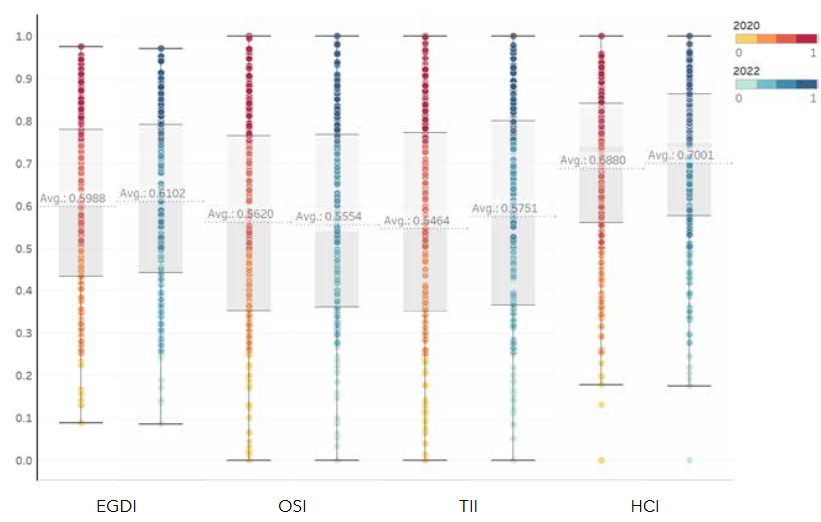
\includegraphics[width=0.7\textwidth]{assets/egdi2020_2022}
    \caption{Valores promedio del EGDI y sus componentes}{Fuente: 2020 and 2022 United Nations E-Government Surveys}
    \label{fig:egdi2020_2022}
\end{figure}

El Gobierno Electrónico brinda muchos beneficios a la población como la eliminación de barreras temporales y espaciales, acceso igualitario a la información, colaboración, aumento en la producción de bienes y servicios, en suma, brinda mayor calidad de vida a la ciudadanía.

Los beneficios se crean para los cuatro actores: Gobierno, Empresas, Ciudadanos y Empleados. Generando cuatro tipos de relaciones (figura \ref{fig:g2all}):

\begin{enumerate}
    \item G2C: Government to Citizen
    \item G2B: Government to Business
    \item G2E: Government to Employee
    \item G2G: Government to Government
\end{enumerate}

\begin{figure}[!h]
    \centering
    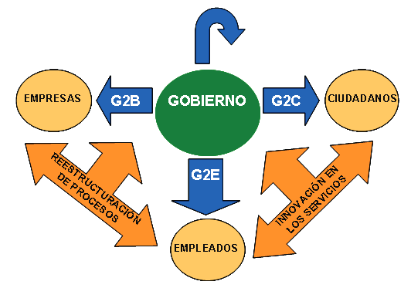
\includegraphics[width=0.7\textwidth]{assets/g2all}
    \caption{Modelo Relacional de Servicios de la Administración Pública}{Fuente: Naser, El Gobierno Electrónico}
    \label{fig:g2all}
\end{figure}

\subsection{Software Libre Reutilizable}

la creación del Sofware FOSS se atribuye a Richard Stallman, conocido como el padre del código abierto. El mismo creía que todos merecían colaborar libre y abiertamente con otros utilizando software, por lo que en 1983 presentó el Proyecto GNU, el cual constituye el primer sistema operativo libre. Posteriormente en 1985 siguió con la creación de la Free Software Foundation para apoyar aún más a la comunidad del software libre. A finales de la década de 1990 el reconocimiento generalizado de Linux y el lanzamiento del código fuente del navegador Netscape aumentó el interés y la participación en el Software libre. La etiqueta de Open Source se creó en una sesión estratégica celebrada el 3 de febrero de 1998 en Palo Alto, California, poco después de que se publicara el código fuente de Netscape. Sin embargo, el término que actualmente se considera más correcto de usar es el de FOSS, ya que acuña ambas definiciones (Free and Open Source Software). 

El software libre es principalmente colaborativo y reutilizable, afectando positivamente a la economía. En un principio, las grandes corporaciones se negaban a apoyar el desarrollo de FOSS. Sin embargo, vista la utilidad del mismo, hoy en día se prefiere su utilización.

El software que se reutiliza es software de mayor calidad y a menores costos económicos y temporales. Implica una gran ventaja sobre los desarrollos desde cero.